\documentclass{article}

%call packages
\usepackage{titlesec}
\usepackage{titling}
\usepackage[margin=.9in, top=0.59in]{geometry}
\usepackage{hyperref}
\usepackage{mathtools}
\usepackage{tabto}
\usepackage{graphicx}
\usepackage{float}
\graphicspath{ {./} }
\usepackage{listings}
\usepackage{color}

\definecolor{codegreen}{rgb}{0,0.6,0}
\definecolor{codegray}{rgb}{0.5,0.5,0.5}
\definecolor{codepurple}{rgb}{0.58,0,0.82}
\definecolor{backcolour}{rgb}{0.95,0.95,0.92}

\lstdefinestyle{mystyle}{
	backgroundcolor=\color{backcolour},   
	commentstyle=\color{codegreen},
	keywordstyle=\color{magenta},
	numberstyle=\tiny\color{codegray},
	stringstyle=\color{codepurple},
	basicstyle=\footnotesize,
	breakatwhitespace=false,         
	breaklines=true,                 
	captionpos=b,                    
	keepspaces=true,                 
	numbers=left,                    
	numbersep=5pt,                  
	showspaces=false,                
	showstringspaces=false,
	showtabs=false,                  
	tabsize=2
}

\lstset{style=mystyle}

%header of document
\title{Twitter Data Analysis}
\author{David Wilson \& Grant Haataja}
\date{\today}
%set paragraph spacing
\linespread{1.5}

\begin{document}
\maketitle

\newpage
%table of contents
\tableofcontents

%format titles for sections, no numbers and no indentation
\titleformat{\section}
{\Large\bfseries}
{}
{0em}
{}

\newpage
%start the hack
\section{Introduction}
\tab A growing concern of social media is the amount of profanity and inappropriate content appearing to the public. This paper will address this issue by outlining data analysis for profanity on Twitter.

\section{Goals of Analysis}
\tab The goals for this analysis were to test the occurrence of profanity from a sample of tweets, to determine whether Twitter was more than 50\% profane or not. But more interestingly, the goal was to find the proportion of tweets that contain profanity. 


\section{Methodology}
\tab ***David Write your stuff here***

\section{Twitter API}
\tab ***David Write your stuff here***

\section{Code to parse .json files}
\lstinputlisting[language=Python]{jsonreader.py}
The following picture shows the output of the above code when ran on the 100 json files that were created from the queries.

\begin{figure}[h]
	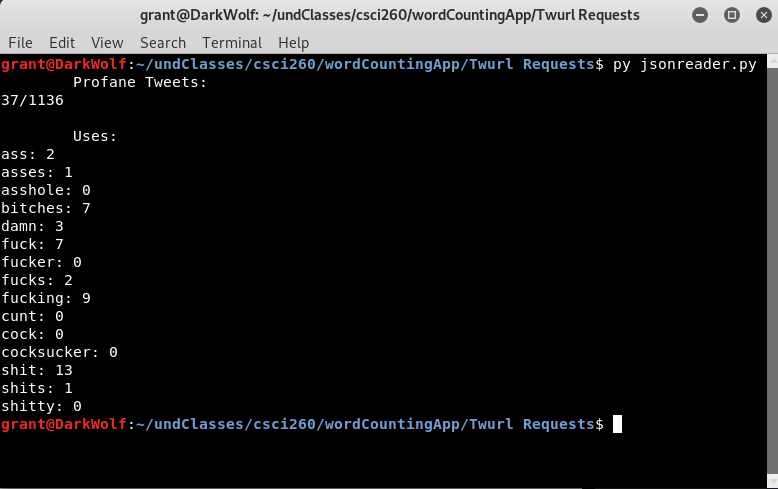
\includegraphics[scale=2.59]{terminal}
\end{figure}

\section{Tweet Examples}
\tab In this section, several of the tweets that were searched are shown. The program did not output the entirety of some of the longer tweets. Note that many of them have multiple occurrences of different profane words, so some of them may be counted twice.\newline

\begin{flushleft}------------------------\newline
rt @quackityhq: fuck koalas why can those little shits sleep 22 hours a day and be seen as cute but when i do it im seen as a lazy piece of…\newline
-------------------------\newline
rt @braindumptweets: trying to figure out how sex works but it doesn't seem plausible, how am i supposed to fit my entire ass in a woman's…\newline
-------------------------\newline
adding arya to my muted words because you bitches can’t be trusted.\newline
-------------------------\newline
rt @iamvee\_: i haven’t been this happy in about 3 fucking years boy\newline
-------------------------\newline
he appears healthy but he seems just to be very damn tired. i'll keep an eye on him and call an animal sanctuary later\newline
-------------------------\newline
if i could get my tubes tied today i fucking would. i’d sell every single one of my eggs. fuck dem kids.\newline
-------------------------\newline
waw i already miss them ;(( my spoiled ass need to stop i keep missing them even if they feed me so much\newline
------------------------\newline
\end{flushleft}

\section{Code to Create Graphs}
\tab Shown below is the Python code used to generate the pie chart used to display the data results.\newline

\lstinputlisting[language=Python]{piechart.py}

The following is the code to generate the bar chart containing the actual number of tweets with the queried profanities.\newline

\lstinputlisting[language=Python]{barchart.py}

\section{The Data}
\tab Below are the recorded percentages of various profanity from the 1136 tweets in the sample size. A total of 37 tweets were found to be profane.

\begin{figure}[h]
	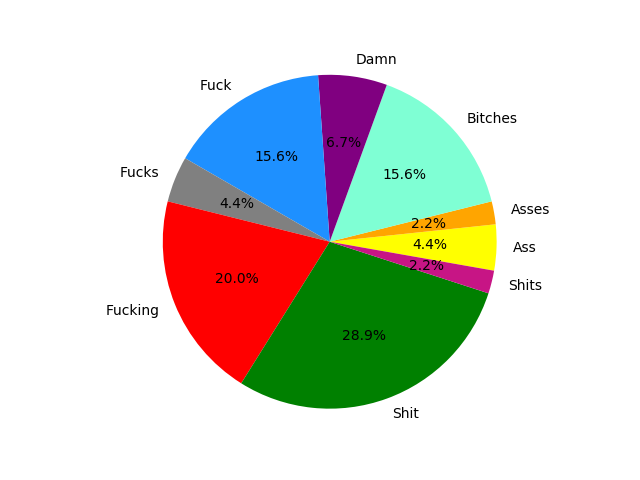
\includegraphics[scale=1]{Figure_1}
\end{figure}

Shown in the next chart are the actual numbers of occurrences of the various profanity in the 37 profane tweets found from the sample.

\begin{figure}[h]
	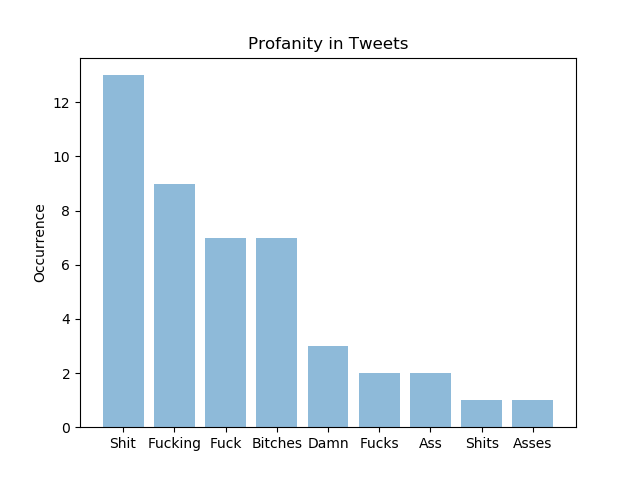
\includegraphics[scale=1]{Figure_2}
\end{figure}

\section{Conclusions}
\tab The data collected show that Twitter is much less profane than 50\%. In fact, only about 3.3\% of tweets collected were found to be profane. However, those that did contain profanity often had multiple occurrences of it. The question of the safety of a platform such as Twitter must ultimately be answered by the individual.

\section{Further Research}
\tab This small data study could be expanded into a much larger research project quite easily by collecting profanity proportions from other social media platforms, and analyzing possible correlations between variables. It would be interesting indeed to see which of the major social media platforms had the most occurrences of profanity, which had the largest total number of profane words, or how the amount of profanity of a platform was correlated to users' opinion of the platform. 

\newpage
\begin{thebibliography}{}
	\bibitem{stuff}I don't think we need any references, do we?

	
	
\end{thebibliography}

\end{document}